\subsection{Magnetic Fields}
\hrulefill

\paragraph*{Definition}
    A magnetic field is a vector field that describes the magnetic influence on moving electric charges, 
electric currents, and magnetic materials. They are generated by moving charges, or current. 
It is represented by the symbol $\vec{B}$ and is measured in teslas (T).\\

    Unlike electric fields, which can be generated by a single source charge, magnetic poles always come in pairs. 
There are no magnetic monopoles. The two types of magnetic poles are called north and south.

\begin{equation*}
    \vec{F}_B = q\vec{v} \times \vec{B}
\end{equation*}

    Where $\vec{F}_B$ is the magnetic force in newtons, $q$ is the charge in coulombs, $\vec{v}$ is the velocity
of the charged in meters per second, and $\vec{B}$ is the magnetic field in teslas.\\

    Note that the magnetic force Insert perpendicular to both the velocity of the charge and the magnetic field. 
This is different from the electric force, which is parallel to the electric field. The direction of the magnetic 
force can be determined using the right hand rule.\\

\begin{center}
    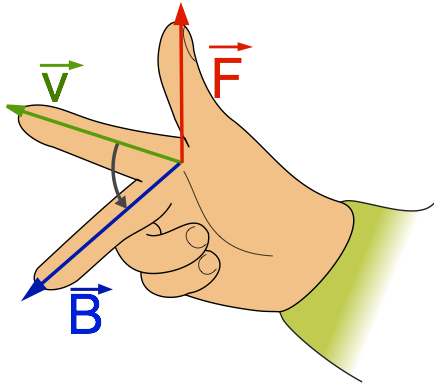
\includegraphics[scale=0.5]{rhr.png}
\end{center}

By convention, $\odot$ represents a vector going into the page, and $\otimes$ represents one coming out of the page.


\paragraph{Charged Particle in a Uniform Magnetic Field}
When a charged particle moves in a uniform magnetic field, it experiences a constant magnetic force that is directed
radially inward. This causes the particle to move in uniform circular motion. We can revise the UCM equations in terms
of the magnetic field and charge of the particle in UCM.

\begin{align*}
    F_B &= qvB = \frac{mv^2}{r}\\
    r &= \frac{mv}{qB}\\
    \omega &= \frac{v}{r} = \frac{qv}{m}\\
    T &= \frac{2\pi r}{v} = \frac{2\pi}{\omega} = \frac{2\pi m}{qB}\\
\end{align*}

Where $F_B$ is the magnetic force in newtons, $q$ is the charge of the particle in coulombs, $v$ is the velocity of the 
particle in meters per second, $B$ is the magnetic field in teslas, $m$ is the mass of the particle in kilograms, $r$ is 
the distance of the particle from the axis of rotation in meters, $\omega$ is the angular velocity in radians per second, 
and $T$ is the period in seconds.\\

\paragraph*{Magnetic Force Acting on a Current-Carrying Wire}
When a current-carrying wire is placed in a magnetic field, it experiences a magnetic force. This force is given by the
following equation.

\begin{align*}
    \vec{F}_B &= I\vec{\ell} \times \vec{B}\\
\end{align*}

Where $\vec{F}_B$ is the magnetic force in newtons, $I$ is the current in amperes, $\vec{\ell}$ is the length of the wire in meters,
and $\vec{B}$ is the magnetic field in teslas. The direction of the force can be determined using the right hand rule.\\

\paragraph*{Torque on a Current Loop in a Magnetic Field}
When a current loop is placed in a magnetic field, it experiences a torque. This torque is given by the following equation.

\begin{align*}
    \vec{\tau}_{mag,dipole} &= \vec{\mu} \times \vec{B}\\
    \vec{\mu} &= I\vec{A}\\
    U_B &= -\vec{\mu} \cdot \vec{B}\\
\end{align*}

Where $\vec{\tau}_{mag,dipole}$ is the torque in newton-meters, $\vec{\mu}$ is the magnetic dipole moment in ampere-square meters,
$B$ is the magnetic field in teslas, $I$ is the current in amperes, and $A$ is the area of the loop in square meters.\\


\paragraph*{Hall Effect}
The Hall effect is the production of a voltage difference (the Hall voltage) across an electrical conductor,
when a magnetic field is applied perpendicular to the current. The Hall voltage is given by the following equation.

\begin{align*}
    E_H &= v_dB = \frac{IB}{nq}\\
    \Delta V_H &= E_H d = \frac{IBd}{nqA} = \frac{IB}{nqt}
\end{align*}

Where $E_H$ is the Hall electric field in volts per meter, $v_d$ is the drift velocity in meters per second, $B$ is the magnetic field in teslas,
$n$ is the number of charge carriers per unit volume in per cubic meter, $q$ is the charge of the particle in coulombs, $I$ is the current in amperes,
$d$ is the thickness of the conductor in meters, $A$ is the cross-sectional area of the conductor in square meters, and $t$ is the time in seconds.\\

\pagebreak

\subsubsection*{Sources of Magnetic Fields}
\hrulefill

\paragraph*{Biot-Savart Law}
The Biot-Savart law describes the magnetic field produced by a current-carrying wire. It is given by the following equation.

\begin{align*}
    d\vec{B} &= \frac{\mu_0}{4\pi}\frac{Id\vec{\ell} \times \hat{r}}{r^2}\\
    \vec{B} &= \frac{\mu_0 I}{4\pi}\int \frac{d\vec{\ell} \times \hat{r}}{r^2}\\
\end{align*}

Where $d\vec{B}$ is the magnetic field in teslas, $\mu_0$ is the permeability of free space in henries per meter (a constant), 
$I$ is the current in amperes, $d\vec{\ell}$ represents an infinitesimal segment of the wire's length, $\hat{r}$ is the unit vector 
pointing from the wire to the point where the magnetic field is being measured, and $r$ is the distance from the wire to the point where 
the magnetic field is being measured in meters.\\

Much like the electric field, the magnetic field generated by an object varies with it's geometry. The two most common geometries are a straight 
wire and a loop of wire.

\begin{align*}
    \vec{B}_{straight} &= \frac{\mu_0 I}{2\pi r}\\
    \vec{B}_{loop} &= \frac{\mu_0 I}{2R}\\
    \frac{\vec{F}_{B\parallel}}{\ell} &= \frac{\mu_0 I_1 I_2 \ell}{2\pi d}
\end{align*}

Where $\vec{B}_{straight}$ is the magnetic field of a straight wire in teslas, $\vec{B}_{loop}$ is the magnetic field of a loop of wire in teslas,
$\mu_0$ is the permeability of free space in henries per meter, $I$ is the current in amperes, $r$ is the distance from the wire to the point where
the magnetic field is being measured in meters, and $R$ is the radius of the loop in meters.\\


\paragraph*{Ampere's Law}
Ampere's Law is similar to Gauss's Law, but for magnetic fields. Unlike Gauss's Law, Ampere's Law is a line integral rather than an area integral. 
It is given by the following equation.

\begin{align*}
    \oint \vec{B} \cdot d\vec{\ell} = \mu_0 I_{enc}
\end{align*}

Where $\vec{B}$ is the magnetic field in Teslas, $d\vec{\ell}$ represents an infinitesimal segment of the wire's length, $\mu_0$ is the 
permeability of free space in henries per meter, and $I_{enc}$ is the current enclosed by the loop in amperes.\\

